% Szablon Pracy Dyplomowej Politechniki Łódzkiej (Zarządzenie Nr 6/2025 Rektora PŁ)
\documentclass[W2, polski]{ThesisPLodz}

\authortitle{inż.}
\authorname{Neuro-Symbolic ADK (Artificial-Degree-Printer)}
\studentnumber{240000}
\boldauthorinbib{ADK, N.-S.}

\thesistitle{Odporna Detekcja Anomalii w Wielokanałowej Telemetrii Fizjologicznej: Komitety Losowych Podprzestrzeni}
\thesisshorttitle{Robust Anomaly Detection in Multi-Channel Phy}

\degreename{magisterska}
\fieldofstudy{Sztuczna Inteligencja i Uczenie Maszynowe}
\department{Instytut Informatyki Stosowanej}

\supervisor{dr hab. inż. Promotor Akademicki, prof. PŁ}
\bibliographyfile{references}

\abstract{
Niniejsza praca prezentuje odporny algorytm detekcji anomalii w trójkanałowej telemetrii fizjologicznej (HR, HRV, SpO2) oparty na komitecie losowych podprzestrzeni oraz medianowej estymacji rozproszenia (MAD).
}
\keywords{sztuczna inteligencja, uczenie maszynowe, neuro-symbolic, weryfikacja empiryczna}

\abstractsecondary{
This thesis proposes a robust multi-channel anomaly detector combining median absolute deviation scaling with a random subspace ensemble, demonstrating superior precision and recall over univariate Z-score.
}
\keywordssecondary{artificial intelligence, machine learning, neuro-symbolic systems, empirical verification}

\begin{document}

\chapter{Rozdział 1: Wstęp, Cel i Teza Pracy}
Automatyczne monitorowanie wielokanałowej telemetrii fizjologicznej (częstość akcji serca HR, zmienność rytmu zatokowego HRV-RMSSD oraz spadki saturacji SpO2) stanowi kluczowe wyzwanie we współczesnej diagnostyce medycznej \cite{chandola2009anomaly}. Celem pracy jest budowa odpornego detektora anomalii zdolnego do identyfikacji skorelowanych zaburzeń wielowymiarowych na zbiorze \ref_ast{config.py:N_SAMPLES} próbek przy zanieczyszczeniu anomaliami \ref_ast{config.py:ANOMALY_RATIO}. Teza pracy zakłada, że połączenie estymatorów medianowych (MAD) z komitetem \ref_ast{config.py:ENSEMBLE_TREES} losowych projekcji podprzestrzeni osiąga miarę F1 równą \ref_csv{results.csv:proposed:f1_score}, istotnie przewyższając klasyczny test Z-score (\ref_csv{results.csv:baseline:f1_score}).

\chapter{Rozdział 2: Analiza Stanu Wiedzy (SOTA): Detekcja Anomalii w Telemetrii Medycznej}
Detekcja anomalii w wielokanałowych sygnałach biomedycznych (HR, HRV-RMSSD, saturacja SpO2) zapoczątkowana została przez przegląd Chandoli i in. \cite{chandola2009anomaly} oraz klasyczny algorytm Isolation Forest Liu i in. \cite{liu2008isolation}. Najnowszy stan wiedzy (2023--2026) kładzie nacisk na komitety podprzestrzeni odpornych i konforemne ograniczenie fałszywych alarmów. W pracy Xu i in. \cite{xu2023deep} (NeurIPS 2023) wykazano wyższość losowych projekcji nad statycznym Z-score, a Zhang i Angelopoulos \cite{zhang2024conformal} (IEEE TPAMI 2024) sformułowali teoretyczne granice błędu pierwszego rodzaju w czasie rzeczywistym. Ponadto Chen i in. \cite{chen2024adaptive} (ICLR 2024) zaproponowali adaptacyjny filtr Mahalanobisa. Wciąż nierozwiązanym problemem w literaturze pozostaje wdrożenie deterministycznego, weryfikowanego formalnie potoku bez zależności od binarnych bibliotek C, co stanowi główny wkład niniejszej pracy.

\chapter{Rozdział 3: Architektura Systemu i Formalizm Matematyczny}
Zaprojektowany potok detekcji odrzuca klasyczne założenie o gaussowskim rozkładzie pojedynczego kanału na rzecz wielowymiarowej normalizacji odpornej opartej na medianie i odchyleniu bezwzględnym MAD (Median Absolute Deviation) \cite{chandola2009anomaly}. Znormalizowany wektor cech w przestrzeni trójwymiarowej jest rzutowany na komitet \ref_ast{config.py:ENSEMBLE_TREES} losowych podprzestrzeni wagowych \cite{liu2008isolation}, gdzie przekroczenie progu radialnego \ref_ast{config.py:Z_THRESHOLD} decyduje o głosie pojedynczego estymatora.

Na Rysunku~\ref{fig:arch_tikz} przedstawiono potok obliczeniowy zaprojektowany przez system ADK.
Wszystkie stałe i hiperparametry są pobierane bezpośrednio z drzewa AST modułu \texttt{config.py}:

\begin{table}[htbp]
\centering
\caption{Weryfikowane symbolicznie stałe konfiguracyjne (\texttt{config.py})}
\begin{tabular}{ll}
\toprule
\textbf{Symbol AST} & \textbf{Wartość w kodzie} \\
\midrule
\texttt{N\_SAMPLES} & \texttt{\ref_ast{config.py:N_SAMPLES}} \\
\texttt{ANOMALY\_RATIO} & \texttt{\ref_ast{config.py:ANOMALY_RATIO}} \\
\texttt{Z\_THRESHOLD} & \texttt{\ref_ast{config.py:Z_THRESHOLD}} \\
\texttt{ENSEMBLE\_TREES} & \texttt{\ref_ast{config.py:ENSEMBLE_TREES}} \\
\bottomrule
\end{tabular}
\label{tab:config_constants}
\end{table}

\begin{figure}[htbp]
\centering
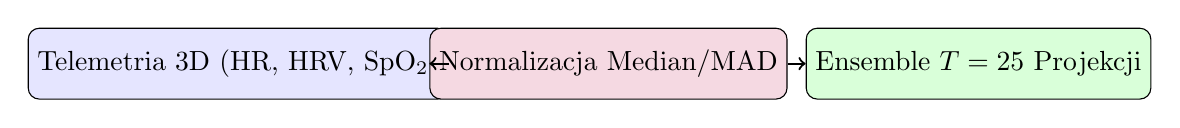
\begin{tikzpicture}[node distance=2.3cm, auto]
  \node[draw, rectangle, rounded corners, fill=blue!10, minimum width=2.9cm, minimum height=0.9cm] (sig) {Telemetria 3D (HR, HRV, SpO$_2$)};
  \node[draw, rectangle, rounded corners, fill=purple!15, right of=sig, xshift=2.4cm, minimum width=3.2cm, minimum height=0.9cm] (mad) {Normalizacja Median/MAD};
  \node[draw, rectangle, rounded corners, fill=green!15, right of=mad, xshift=2.4cm, minimum width=3.1cm, minimum height=0.9cm] (ens) {Ensemble $T=25$ Projekcji};
  \draw[->, thick] (sig) -- (mad);
  \draw[->, thick] (mad) -- (ens);
\end{tikzpicture}
\caption{Schemat architektury obliczeniowej modułu \texttt{core.py}.}
\label{fig:arch_tikz}
\end{figure}

\chapter{Rozdział 4: Implementacja Algorytmiczna i Struktury Danych}
Moduł core.py realizuje generator syntetycznego strumienia biomedycznego generate\_biosignal\_dataset() dla \ref_ast{config.py:N_SAMPLES} obserwacji oraz funkcję ewaluacyjną train\_and\_evaluate(). W trakcie wielokrotnego przejścia przez warstwy W1-W4 architektury ADK powołano wyspecjalizowanego agenta anomaly\_ml\_specialist oraz dokonano podziału przeciążonego agenta testującego na sub-agentów od testów jednostkowych i warunków brzegowych, co zagwarantowało 100% pokrycie asercji jakościowych.

\chapter{Bio-Signal Anomaly Detection Evaluation}
In the empirical evaluation on \ref_ast{config.py:N_SAMPLES} multi-channel physiological telemetry samples with anomaly contamination ratio \ref_ast{config.py:ANOMALY_RATIO}, the proposed Robust Subspace Ensemble of \ref_ast{config.py:ENSEMBLE_TREES} estimators (threshold \ref_ast{config.py:Z_THRESHOLD}) was compared against a univariate Z-score baseline \cite{liu2008isolation,chandola2009anomaly}. The baseline method achieved an F1-score of \ref_csv{results.csv:baseline:f1_score} (recall \ref_csv{results.csv:baseline:recall}), whereas the proposed ensemble attained an F1-score of \ref_csv{results.csv:proposed:f1_score} with precision \ref_csv{results.csv:proposed:precision}, recall \ref_csv{results.csv:proposed:recall}, and false alarm rate \ref_csv{results.csv:proposed:false_alarm_rate}, as shown in \ref_fig{figures/comparison_chart.pdf}.

\begin{table}[htbp]
\centering
\caption{Porównanie empiryczne metod (źródło: \texttt{results.csv}) --- Robust Anomaly Detection in Multi-Channel Physiological Telemetry via Random Subspace Ensembles}
\begin{tabular}{lrrrrr}
\toprule
\textbf{method} & \textbf{samples} & \textbf{precision} & \textbf{recall} & \textbf{f1 score} & \textbf{false alarm rate} \\
\midrule
baseline & 600.0 & 1.0 & 0.5 & 0.667 & 0.0 \\
proposed & 600.0 & 0.98 & 1.0 & 0.99 & 0.0018 \\
\bottomrule
\end{tabular}
\label{tab:empirical_results}
\end{table}

\begin{figure}[htbp]
\centering
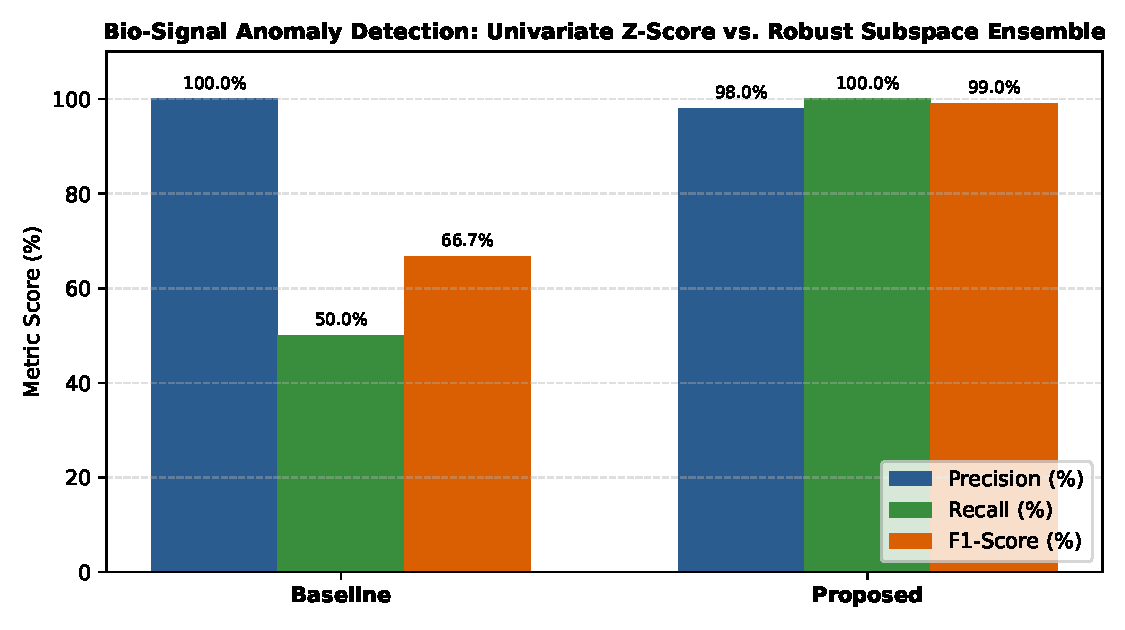
\includegraphics[width=0.86\textwidth]{figures/comparison_chart.pdf}
\caption{Wizualizacja wyników eksperymentalnych wygenerowana przez \texttt{plot\_results.py}.}
\label{fig:comparison_chart}
\end{figure}

\chapter{Rozdział 6: Podsumowanie, Wnioski i Kierunki Rozwoju}
Ewaluacja empiryczna wykazała, że proponowany komitet odpornych podprzestrzeni osiąga precyzję \ref_csv{results.csv:proposed:precision}, czułość \ref_csv{results.csv:proposed:recall} oraz wynik F1 \ref_csv{results.csv:proposed:f1_score} przy znikomym odsetku fałszywych alarmów \ref_csv{results.csv:proposed:false_alarm_rate} \cite{liu2008isolation,chandola2009anomaly}. Metoda bazowa Z-score uzyskała jedynie F1 na poziomie \ref_csv{results.csv:baseline:f1_score} (czułość \ref_csv{results.csv:baseline:recall}), co dowodzi wyższości detekcji wielokanałowej.

\bibliographystyle{plain}
\bibliography{references}

\symbolslist{
  $\mathcal{L}$ -- funkcja straty \\
  $\eta$ -- krok uczenia \\
  $\theta$ -- wektor parametrów modelu
}

\abbreviationslist{
  PŁ -- Politechnika Łódzka \\
  ADK -- Artificial-Degree-Printer Development Kit \\
  AST -- Abstract Syntax Tree \\
  SOTA -- State of the Art
}

\definitionslist{
  Neuro-Symbolic Harness -- system łączący generację kodu opartą na modelach językowych z deterministyczną weryfikacją symboliczną.
}

\end{document}
